\documentclass[10pt]{article}
\usepackage[pdftex]{graphicx} 
\usepackage[comma,numbers,sort&compress]{natbib} % round/square, authoryear/numbers
\usepackage{amsfonts,amsmath,amssymb,amsthm} % various math stuff
% \usepackage[compact]{titlesec}  % Allow compact titles
\usepackage{sectsty} % Allows for section style to be manipulated
\usepackage{wrapfig}  % Allow wrapping of text around figures
\usepackage{mdwlist}  % Make list items closer together: itemize*, enumerate*
\usepackage{sidecap}  % For putting caption beside figure
\usepackage{bm} % for bold math (via \boldsymbol or \pbm)
\usepackage{xcolor}
\usepackage[colorlinks=true, allcolors=blue]{hyperref} % For hyper-linked refs and bib

\usepackage[toc]{appendix}

% ==  FONT  ===========================
% ---- uncomment for Helvetica (sansserif)  -------------
\usepackage[T1]{fontenc}
\usepackage[scaled]{helvet}
\renewcommand*\familydefault{\sfdefault}  % If the base font of the document is to be sans serif

% ======= File locations =================
\input{latexstuff/jpdefs} % define some useful latex commands
\newcommand{\figdir}{figs}  % fig directory
\newcommand{\mybibfile}{latex/jpbib}  % bib files 


% ----- Float (figure) positioning --------------------------------------
\setcounter{topnumber}{1}  % max # floats at top of page
\setcounter{bottomnumber}{1} % max # at bottom of page
\setcounter{totalnumber}{1} % max floats on a page
\renewcommand{\topfraction}{1} % max frac for floats at top
\renewcommand{\bottomfraction}{1} % max for floats at bottom
\renewcommand{\textfraction}{0} % minimum fraction of page for text
%\setlength{\textfloatsep}{.2in}  % separation between figure and text

% ---- Control paragraph spacing and indenting  -------------------
\setlength{\textheight}{9in} % 11 - ( 1.5 + \topmargin + <bottom-margin> )
\setlength{\textwidth}{6.5in} % 8.5 - 2 * ( 1 + \oddsidemargin )
\setlength{\topmargin}{0in}  % in addition to 1.5'' standard margin
\setlength{\oddsidemargin}{0in} % in addition to 1'' standard
\setlength{\parindent}{0em}  % indentation 
\setlength{\parskip}{1.5ex} % paragraph gap 
\setlength{\headsep}{0.0in}
\setlength{\headheight}{0.0in}
%\renewcommand\baselinestretch{0.94}\large\normalsize 

% %% OTHER COMMANDS ------------------------------------------------

\newcommand{\vx}{\mathbf{x}}
\newcommand{\vxto}{\mathbf{x}_{t+1}}
\newcommand{\vw}{\mathbf{w}} 
\newcommand{\vy}{\mathbf{y}}
\newcommand{\vm}{\mathbf{m}} 
\newcommand{\vv}{\mathbf{v}}
\newcommand{\vu}{\mathbf{u}}
\newcommand{\mvec}{\mathrm{vec}}
\newcommand{\mH}{\mathbf{H}}
\newcommand{\mQ}{\mathbf{Q}}
\newcommand{\tmQ}{\mathbf{\tilde Q}}
\newcommand{\mLam}{{\mathbf{\Lambda}}} 
\newcommand{\mSig}{{\mathbf{\Sigma}}}
\newcommand{\mR}{\mathbf{R}}
\newcommand{\mC}{\mathbf{C}}
\newcommand{\Pinf}{P_\infty}
\newcommand{\trpinv}{^{-\!\top}}
\newcommand{\cov}{\mathrm{cov}}  
\renewcommand{\RR}{\mathbb{R}}
% \newcommand{\inv}{^{-1}}
% \newcommand{\Tr}{\mathrm{Tr}}


% Change equation numbering
% \numberwithin{equation}{section}
% \renewcommand{\theequation}{\thesection.\arabic{equation}}

\raggedbottom
\allowdisplaybreaks


\title{A tutorial overview of the Kalman filter and latent linear
  dynamical systems}
\author{Jonathan W. Pillow \\
  Princeton Neuroscience Institute \\
  Princeton University \\
  {\texttt{http://pillowlab.princeton.edu}}}


%----------------------------------------------------------------
\begin{document}


\maketitle

\tableofcontents
\newpage
% % % --- Publication note ---------
% \vbox to 0.2in{ \vspace{-3.25in}
% \small\tt  Draft Information}


\setspacing{1.1}
\centerline{\textbf{Abstract}}
\hbox to \textwidth{\hrulefill} 
%\vspace{-.1in}

% --- Abstract -------------------------------------------------------------------------
This paper provides a tutorial introduction to the Kalman filter and
the generative model associated with it: the Gaussian latent linear dynamical system.   
\\
\hbox to \textwidth{\hrulefill}


%--------------------------------------------------------------------------

\setspacing{1}

\section{Introduction}



In this tutorial, we will introduce Gaussian latent linear dynamical
system (LLDS) models and derive
the classic Kalman filtering and smoothing algorithms.   We will then
derive the expectation-maximization algorithm for fitting the
parameters of a Gausian LLDS model to data.

In the appendix, we provide several additional derivations, such as
external inputs, multiple trials, missing data, and an alternate implementations involving block-sparse matrices.

The Kalman filter, also known as the Kalman-Bucy filter
\cite{Kalman60,KalmanBucy1961}, was first derived from the perspective
of least squares, with no explicit connection to Bayesian inference.
For more on the origins of the Kalman filter see
\cite{SarkkaBook2013}.


\subsection{Notation}

We will use $\Nrm(\vx; \mu,\Sigma)$ to denote a multivariate normal
probability density function over $\vx$ with mean $\mu$ and variance
$\Sigma$.  When it is obvious what the variable in question is, we
will abbreviate this more simply as $\Nrm(\mu,\Sigma)$. 

{\it To do: flesh this out.}

\section{The Latent Linear Dynamical System (LLDS) model} %---------------------------%


Consider the latent linear dynamical system (LLDS) defined by:
\begin{alignat}{5}
  \label{eq:latent}
  \vx_{t} &=\;&& A \vx_{t-1} &&+ \vw_t, \qquad && \vw_t \sim \Nrm(0,Q)
  \qquad  && \text{\it(latent dynamics)}\\
    \label{eq:obs}
  \vy_{t} &=\;&& C \vx_t &&+ \vv_t, \qquad && \vv_t \sim \Nrm(0,R) && 
  \text{\it(observations)}
\end{alignat}
Here $\vx_t \in \RR^m$ is a ``latent'' or ``unobserved'' vector, also commonly known as the state vector, and 
$\vy_t\in\RR^n$ is the ``observed'' or ``measured'' or ``output'' vector, also known as the ``emissions''.  The noise vectors $\vw_t \in \RR^m$ and $\vv_t\in \RR^n$ denote samples of zero-mean
Gaussian noise, which corrupt the latent state and the observations,
respectively.  In the control literature, this model is commonly known as a {\it discrete-time state-space linear system} \cite{HespanhaBook}.

In the Gaussian LLDS model, the latent vector $\vx_t$ evolves linearly according to an $m\times m$ dynamics matrix
$A$.  The observations $\vy_t$ result from a linear function of 
$\vx_t$ via the observation matrix $C$. To give the model a
well-defined initial state, we add a prior over the latent vector at time
step one:
\begin{equation}
  \label{eq:initial}
  \vx_1 \sim \Nrm(0, Q_0). \qquad \text{\it (initial latent) }
\end{equation}

Typically we have $m<n$, so that the high-dimensional observations
$\vy_t$ are explained by the lower-dimensional $\vx_t$.
The LLDS model parameters are thus given by
\begin{equation}
  \label{eq:theta}
  \theta = \{A,C,Q,R,Q_0\}, 
\end{equation}
consisting of linear dynamics matrix $A$, observation matrix $C$,
latent noise covariance $Q$, observation noise covariance
$R$, and initial latent covariance
$Q_0$. Fig.~\ref{fig:graphicalmodel} shows an illustration of the LLDS
model, depicted either as a graphical model (left) or a set of matrix
equations (right).


% --- Fig 1: schematic
\begin{figure}[t]
%\begin{
\centering 
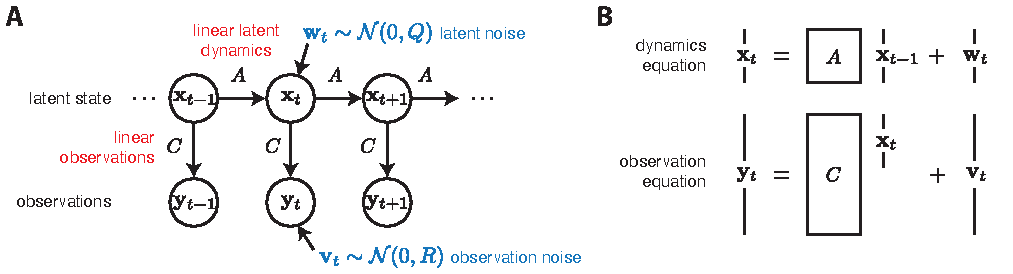
\includegraphics[width=.975\textwidth]{figs/KFgraphicalmodel5}
\caption{Graphical model and equations for a Gaussian latent linear
  dynamical system (LLDS) model, also known as the Kalman filtering model.}
\label{fig:graphicalmodel}
\end{figure}


\subsection{Identifiability}
\label{subsec:identifiability}

Because the latent variables are not observed, a Gaussian LLDS model
is only identifiable up to a linear transformation of its latent
space.  To see this, consider a LLDS model with parameters
${A, C, Q, R, Q_0}$.  Now let us define a new latent variable $\vx_t'$
that is related to the latent variables of the original model by an
invertible linear transformation:
\begin{equation}
  \label{eq:11}
  \vx_t' = H \vx_t,
\end{equation}
for some invertible $m \times m$ matrix $H$. Then we can create a new
LLDS model with parameters
\begin{alignat}{2}
  \label{eq:20}
  A' &= H A H\inv, \quad & 
  C' &= C H\inv, \\
  Q' &= H Q H\trp, \quad & 
  Q_0' &= H Q H\trp,
\end{alignat}
and noise covariance $R$ unchanged.  This new model assigns the same
probability to the observed data as the original model.  This is easy
to see by substituting the linearly transformed latent variable $H \vx_t$ into the system equations
(eq.~\ref{eq:latent}-\ref{eq:initial}) for the new model.

One implication of this non-identiability is that we can transform an
LLDS model in order to simplify its parameters, or increase the
interpretability of its latents, without changing the model. (That is, the parameters of the model can be transformed without having any effect on the probability assigned to the observed data).  For
example, we can transform by $H = Q^{-\tonehlf}$, so that the new dynamics
noise covariance $Q'$ is the identity.  If we wish to make $C$
semi-orthogonal, so its columns are orthogonal unit vectors, we could
transform by $H\inv = V S\inv$, where
$C = U S V\trp$ is the singular value decomposition (SVD) of the
original $C$ matrix, resulting in $C' = U$. 

Note that we are restricted to transforming the
dynamics matrix $A$ to a similarity transformation of itself, since
$A= H A H\inv$. Thus we cannot alter the eigenvalues of $A$, and we
generally cannot diagonalize $A$ if it has complex eigenvalues.  Note also that
such lienar transformations of the latent space do {\it not} allow us to alter the column space
of $C$, or to modify the noise covariance $R$ in any way.


\subsection{Stability and asymptotic behavior}

The stability of an LLDS model is determined by the eigenvalues of the
dynamix matrix $A$, which are in general complex valued.  The
imaginary component of each eigenvalue gives rise to rotations or
oscillations along an associated pair of eigenmodes, while the
absolute value of the eigenvalues determines stability.

If the modulus or absolute value of any eigenvalue exceeds one,
i.e., $\max(\mathrm{abs}(\mathrm{eig}(A)))>1$, then the LLDS is
unstable. This means that if we simulate the model, the latent vector
will diverge exponentially or ``explode''.

By contrast, if all eigenvalues have absolute value less than one,
$\mathrm{max}(\mathrm{abs}(\mathrm{eig}(A)))<1$, then the LLDS model
is stable.  In this regime, the noiseless LLDS model, in which $Q=0$,
will have a latent state that converges to a stable fixed point at 0.
If the latent noise is non-zero, however, then the latent state has a
stable asymptotic Gaussian distribution with mean 0 and covariance
$V_\infty$, where this asymptotic covariance can be computed as the
solution to the discrete Lyapunov equation:
\begin{equation}
  \label{eq:17}
  V_\infty = A V_\infty A\trp + Q.
\end{equation}
In this case, the observations will also have a marginally Gaussian
distribution with mean zero and covariance $C V_\infty C\trp + R$.
(Thus, a simple sanity check when simulating an LDS model or fitting
an LDS model to data is to examine whether the sample covariance of
the data, $\cov(\vy_t \vy_t\trp)$ is close to $C V_\infty C\trp +R$,
where a discrete Lyapunov equation solver is used to obtain $V_\infty$
from $A$ and $Q$.)

Finally, if any eigenvalue has absolute value equal to 1, the
noiseless LLDS model has neutral stability, meaning that it neither
diverges nor converges to zero.  If the covariance $Q$ is
non-singular, moreover, the variance along the associated subspace
grows linearly with time.  Thus, data generated by the model does not possess a
stationary distribution.

\section{Inferring the latents: Kalman filter and smoother}

Kalman filtering is an algorithm for computing the posterior
distribution over latent $\vx_t$ given $\vy_{1:t}$, the observations
from time bin 1 to time $t$.  Kalman filtering is a ``foward''
filtering equation that operates by iteratively updating the posterior
over $\vx_t$ using the data from each time point (see Fig.~\ref{fig:KFvsKS}A).

By contrast, {\it Kalman smoothing} involves propagating information
backwards from the final time step $T$ in order to update the
posterior over $\vx_t$ at all previous times. It corresponds to a
``backwards'' filtering operation that starts at time $T$ and
propagates information iteratively to the latent variable at each
previous time steps (see Fig.~\ref{fig:KFvsKS}B).

% --- Fig 2: Kalman & Smoothing  ----------------
\begin{figure}[t]
\centering 
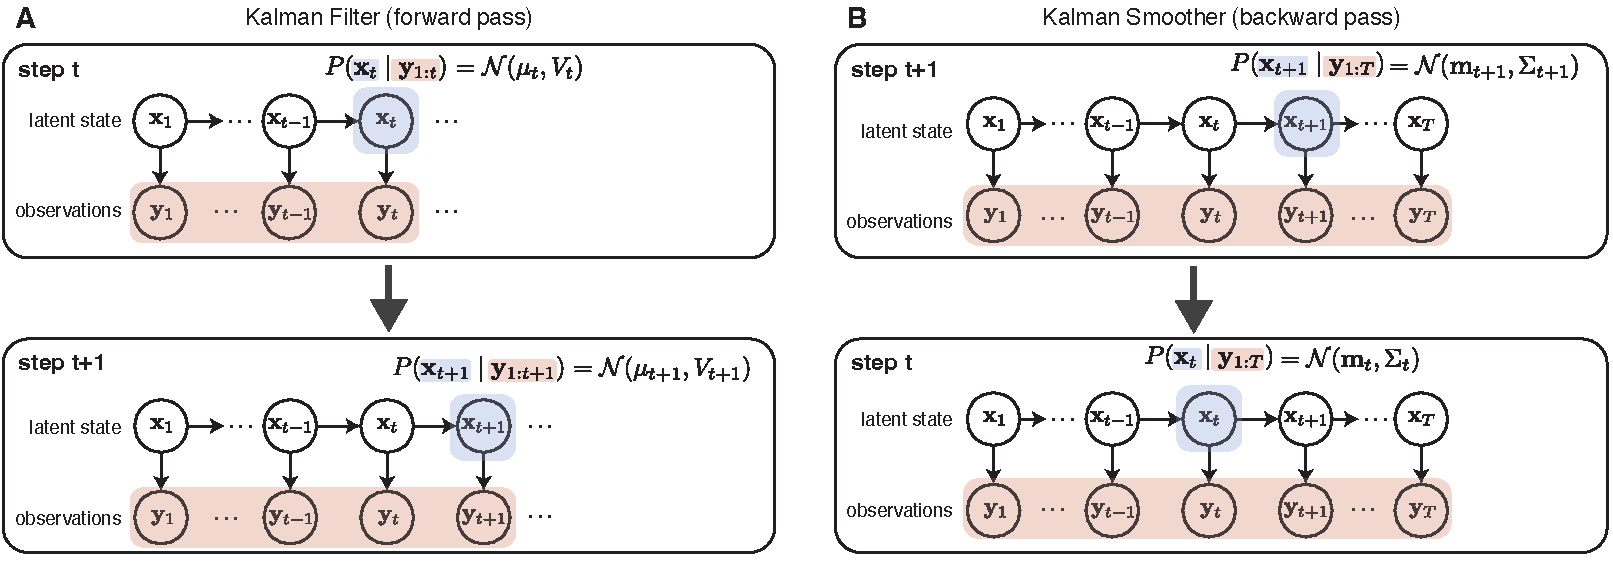
\includegraphics[width=\textwidth]{figs/Filtering_vs_Smoothing_v2.pdf}
\caption{Comparison between Kalman filtering (A) and Kalman smoothing (B).}
% \caption{Illustration of one step of the Kalman filter, which takes
%   $P(\vx_t \mid \vy_{1:t})$ and computes $P(\vx_{t+1} \mid \vy_{1:t+1})$.}
\label{fig:KFvsKS}
\end{figure}

% --- Fig 3: Kalman Filter Steps ------------------
\begin{figure}[t]
\centering 
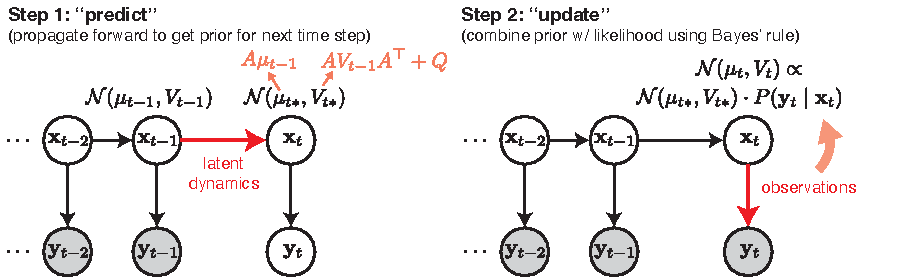
\includegraphics[width=.95\textwidth]{figs/KFsteps_v2}
\caption{Two steps in the kalman filter.}
\label{fig:KF}
\end{figure}


\subsection{Kalman filter}
\label{sec:KF}

The Kalman Filter is a recursive algorithm for computing
$P(\vx_t\mid \vy_{1:t})$, the posterior over the latent state at time
$t$ given all the data up to and including time $t$, from
$P(x_{t-1}\mid \vy_{1:t-1})$ the posterior over the latent at the
previous time step, given the model parameters $\theta$.  The
resulting distribution is necessarily Gaussian, allowing us to write:
\begin{equation}
  \label{eq:16}
  P(\vx_t \mid \vy_{1:t}) =\Nrm(\mu_t, V_t),
\end{equation}
parametrized by a mean $\mu_t$ and covariance $V_t$. Note that $\mu_t$
is also the least-squares estimate of the signal $\vx_t$ given the
data up to time $t$.


% This is also the posterior over the latent
% given previous observations, given that there are no previous
% observations at time step zero. Thus we have posterior means
% $\mu_0 = 0$ and covariance $V_0 = Q_0$ for the initial step of the
% Kalman filter.

% The Kalman filter then proceeds recursively to compute the Gaussian
% distribution over the latent given previous observations.  Given
% $\Nrm(\mu_{t-1},V_{t-1})$, the posterior over the latent state at time
% at time step $t-1$, it computes $\Nrm(\mu_t,V_t)$, the posterior over
% the latent variable at time $t$ while incorporating the observation
% $y_t$.

The recursive update rule for the Kalman filter can then be broken down into two steps (see Fig.~\ref{fig:KF}):\\

{\bf Step 1 (Prediction)}.  The ``prediction'' step of the Kalman
filter takes $P(\vx_{t-1} \mid \vy_{1:t-1})$, the posterior over the
latent at time $t-1$ given observations from 1 to $t-1$, and
propagates it one time step forward using the linear dynamics $A$ and
the latent ``innovations'' noise covariance $Q$. This produces the
{\it prior} over the latent state at time $t$ given the observations
from time step 1 up to $t-1$:
\begin{alignat}{2}
P(\vx_{t}\mid \vy_{1:t-1}) &= \Nrm(\mu_{t*}, V_{t*}),   \quad  & &
\text{\it (Kalman filter prior)} \label{eq:KFprior} \\
\intertext{where}
\mu_{t*} &=  A \mu_{t-1}, \quad  & & \text{\it
  (prior mean)} \label{eq:KFpriormean}
\\
 V_{t*} &= AV_{t-1}A\trp + Q, \quad & & \text{\it (prior covariance)} \label{eq:KFpriorcov}
\end{alignat}
which follow from Gaussian fun facts for linear and additive
transformations of a Gaussian distribution 
(eqs.~\ref{eq:gffsum}-\ref{eq:gfflin}).
The only exception  is that on the very first time
step we have no previous observations, thus the prior is simply:
\begin{equation}
  \label{eq:kfprior1}
P(\vx_1) = \Nrm(0,Q_0),  \qquad   \text{\it (Kalman filter prior, first
  time bin)}
\end{equation}
thus we have that $\mu_{1*}=0$ and $V_{1*} = Q_0$.

% Note that for the first time step, we have
% \begin{equation}
%   \label{eq:10}
%   P(\vx_1 ) = \Nrm(\mu_{1*}, V_{t*}), 
% \end{equation}
% with $\mu_{1*} = 0$ and $V_{t*} = AQ_0Q\trp + Q$, which follows from
% the prior over the initial latent: $\vx_0 \sim \Nrm(0,Q_0)$.


{\bf Step 2 (Update)}.  The second step of the Kalman filter is the
``update'' step, which incorporates information from the observation
$\vy_t$ about the latent $\vx_t$.  This involves using Bayes' rule to
combine the likelihood term $P(\vy_t | \vx_t)$ with the prior
$P(\vx_t | \vy_{1:{t-1}})$ computed in the prediction step. The
product of these two terms is proportional to
$P(\vx_t \mid \vy_{1:t})$, the posterior distribution for time step
$t$. From Bayes' rule, we have:
\begin{alignat}{2}
  P(\vx_{t}\mid \vy_{1:t}) & \propto  P(\vy_{t}\mid \vx_{t}) 
P(\vx_{t}\mid \vy_{1:t-1})
 = \Nrm(\vy_{t};
 C\vx_{t},R) \Nrm(\vx_{t}; \mu_{t*}, V_{t*}).
   \label{eq:BayesKF} 
 \end{alignat}
 Because both prior and likelihood are exponentiated quadratic forms in
 $\vx_t$, we can use Gaussian identities (eq.~\ref{eq:gfflingauss}) to
 obtain the Gaussian form of the posterior distribution:
\begin{equation}
P(\vx_{t}\mid \vy_{1:t}) = 
\Nrm(\mu_{t}, V_{t})
\qquad \text{\it(Kalman filter output)}
  \label{eq:KF}
\end{equation}
where
\begin{alignat}{2}
  \mu_{t} &= V_{t}(C\trp R\inv \vy_{t} + V_{t*}\inv \mu_{t*}),
 \qquad & &  \text{\it (Kalman filter mean)}  \label{eq:KFmean} 
 \\ 
V_{t} &= (V_{t*}\inv + C\trp R\inv C)\inv.
& & \text{\it (Kalman filter covariance)} 
\label{eq:KFcov} 
\end{alignat}


\subsubsection*{Marginal likelihood}
Note that the normalizing constant in the application of Bayes' rule
above (eq.~\ref{eq:BayesKF}) corresponds to
$P(\vy_t \mid \vy_{1:t-1})$, the marginal probability of the
observation $\vy_t$ given all previous observations.  This quantity
can also be derived by noting that $\vy_t$ is a linear transformation
of $\vx_t$ plus Gaussian noise with covariance $R$.  From the prior
over $\vx_t$ (eq.~\ref{eq:KFprior}) and Gaussian fun facts
(eq.~\ref{eq:gffsum}-\ref{eq:gfflin}), we obtain the following expression
for the conditional marginal likelihood:
\begin{equation}
  \label{eq:margliterms}
P(\vy_t \mid \vy_{1:t-1}) = \Nrm(\vy_t; C\mu_{t*}, CV_{t*}C\trp + R), 
\end{equation}
where $\mu_{t*}$ and $V_{t*}$ are the prior mean and variance of the
latent at time step $t$ (eqs.~\ref{eq:KFpriormean}-\ref{eq:KFpriorcov}).

The marginal probability of the entire dataset is given by the product of these
terms:
\begin{equation}
  \label{eq:margli}
  P(\vy_{1:T})  = P(\vy_1) \prod_{t=2}^T P(\vy_t \mid \vy_{1:t-1}), 
\end{equation}
where $P(\vy_1) =
\Nrm(\vy_1; 0, C Q_0 C\trp +R)
= \Nrm(\vy_1; C\mu_{1*}, C V_{1*} C\trp + R)$ is the distribution of
the first observation, with prior mean $\mu_{1*} = 0$.

The log marginal likelihood can therefore be fully computed during the
forward pass of the Kalman filter, without needing the backward pass
of the Kalman smoother (which we discuss below).  We obtain:
\begin{equation}
  \label{eq:logmargli}
  \log P(\vy_{1:T}) = -\tonehlf \sum_{t=1}^T \Big(
  \log |2\pi (CV_{t*}C\trp + R)| + 
  (\vy_t- C \mu_{t*})\trp (CV_{t*}C\trp+R)\inv   (\vy_t- C
  \mu_{t*})\Big).
  %-\tfrac{T}{2} \log (2\pi).
\end{equation}
%where (to simplify notation) we define $\mu_{1*} = \mu_0$ and $V_{1*} =
%V_0$. 

% % ------------------ Kalman Smoother Fig ----------------
% \begin{figure}[h]
% \centering 
% 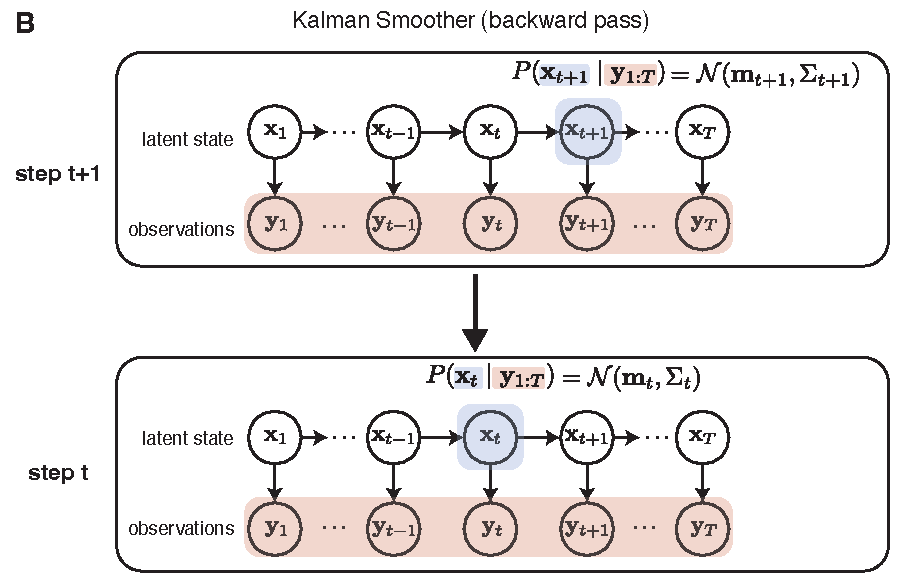
\includegraphics[width=.65\textwidth]{figs/Fig_KSmoothing}  
% \caption{Comparison between Kalman filtering (A) and Kalman smoothing (B).}
% \label{fig:KFvsKS}
% \end{figure}


\subsection{Kalman Smoother}
\label{sec:ksmooth} 
The Kalman Smoother represents the ``backwards'' complement to the
Kalman Filter. The Kalman filter marches forward in time to update the
posterior over the latent variable given {\it past} observations; the
Kalman smoother, by contrast, marches backward in time to update the
posterior over the latents with information about {\it future}
observations.

Because these distributions are Gaussian, the Kalman smoother amounts
to an algorithm for updating the mean and covariance of the latent
given future observations. Thus the Kalman smoother produces:
\begin{equation}
  \label{eq:15}
  P(\vx_t \mid \vy_{1:T}) = \Nrm( \vm_t, \Sigma_t),  
\end{equation}
where $\vm_t$ and $\Sigma_t$ are the mean and covariance of the
posterior distribution over the latent vector at time bin $t$.

The Kalman smoother begins at time step $T$, where the Kalman filter
terminates.  The posterior over the latents at $T$ is obtained
direclty from the last step of the Kalman filter, thus we have:
\begin{equation}
 P(\vx_T \mid \vy_{1:T}) = \Nrm(\vm_T, \Sigma_T) = \Nrm(\mu_T, V_T).
\end{equation}

The Kalman then proceeds recursively, taking
$P(\vx_{t+1} \mid \vy_{1:T})$, the posterior over $\vx_{t+1}$ given
all observations from past and future, and propagating it one step
backwards in time to obtain $P(\vx_t \mid \vy_{1:T})$.  This requires
combining future information from $\vy_{t+1:T}$ with past information
from $\vy_{1:t}$ computed via the Kalman filter.

To see how this can be accomplished, we start by writing the posterior
over $\vx_t$ as the marginalization of joint posterior over $\vx_t$
and $\vx_{t+1}$:
\begin{align}
  P(\vx_t \mid \vy_{1:T}) &=  \int P(\vx_t,\vx_{t+1} \mid \vy_{1:T})\,
       d\vx_{t+1} \label{eq:ks1}
  \\
                        &= \int P(\vx_t \mid \vx_{t+1}, \vy_{1:T})\,
                          P(\vx_{t+1} | \vy_{1:T}) \, d\vx_{t+1}
\label{eq:ks2}
  \\
                        &= \int P(\vx_t \mid \vx_{t+1}, \vy_{1:t})\,
                          P(\vx_{t+1} | \vy_{1:T}) \, d\vx_{t+1},
                          \label{eq:ks3} \\
  & =  \int P(\vx_t \mid \vx_{t+1}, \vy_{1:t})\,
                          \Nrm(\vx_{t+1}; \vm_{t+1}, \Sigma_{t+1}) \,
    d\vx_{t+1},
             \label{eq:ks4}
\end{align}
where (eq.~\ref{eq:ks2}) is simply an application of the definition of
conditional probability, and (eq.~\ref{eq:ks3}) follows from the fact
that $\vx_t$ is conditionally independent of future observations
$\vy_{t+1:T}$ given $\vx_{t+1}$, meaning that
$P(\vx_t \mid \vx_{t+1}, \vy_{1:T}) = P(\vx_t \mid \vx_{t+1},
\vy_{1:t})$.  In  (eq.~\ref{eq:ks4}), we have simply substituted the
Gaussian from the previous step of the Kalman smoother for
$P(\vx_{t+1} \mid \vy_{1:T})$. 

The first term in (eq.~\ref{eq:ks4}),
$P(\vx_t \mid \vx_{t+1}, \vy_{1:t})$, can be obtained from terms
computed during the forward pass of the Kalman filter, since it
involves only past observations $\vy_{1:t}$.  To compute it, we can
start by deriving the joint distribution
$P(\vx_{t}, \vx_{t+1} \mid \vy_{1:t})$.  From the Kalman filtering
equations (eqs.~\ref{eq:KFprior}-\ref{eq:KFpriorcov}), the joint
distribution over a pair of adjacent latent states given previous
observations is:
\begin{align}
  \label{eq:8}
  P \left( \begin{bmatrix}
    \vx_t \\
    \vxto
  \end{bmatrix} \mid \vy_{1:t} \right) 
    \; = \; \Nrm \left(
  \begin{bmatrix}
    \mu_t \\ A \mu_t 
  \end{bmatrix}, 
  \begin{bmatrix}
    V_t & V_t A\trp \\
    A V_t & A V_t A\trp
   \end{bmatrix} \right)
\;  =\; \Nrm \left(
  \begin{bmatrix}
    \mu_t \\ \mu_{t+1*} 
  \end{bmatrix}, 
  \begin{bmatrix}
    V_t & V_t A\trp \\
    A V_t & V_{t+1*}
  \end{bmatrix} \right),
%
\end{align}
where $\mu_{t+1*}$ and $V_{t+1*}$ in the right-most expression denote
the prior mean and covariance over $\vxto$ given the data up to time
bin $t$. We can then apply the Gaussian fun fact for
conditionalization (eq.~\ref{eq:gffcond}) to obtain:
\begin{equation}
  \label{eq:7}
  P(\vx_t \mid \vxto, \vy_{1:t} )  = \Nrm( \mu_t + V_t A\trp
  V_{t+1*}\inv (\vxto - \mu_{t+1*}), V_t - V_t A\trp V_{t+1*}\inv A
  V_t ).
\end{equation}
Note that this is equivalent to writing:
%\begin{alignat}{3}
%  \label{eq:9}
%  \vx_t
  %&= (V_t A\trp V_{t+1*}\inv) \vxto & \;+\;& \mu_t  - (V_t 
%  A\trp V_{t+1*}\inv) \mu_{t+1*} &\;+\;& \textrm{noise} \\
%&= J_t\, \vxto &\;+\;& \mu_t  - J_t \mu_{t+1*}  &\;+\;& \textrm{n}, \\
% \end{alignat}
% ----------------
\begin{equation}
  \label{eq:12}
    \vx_t =  \mu_t  + J_t (\vxto    -  \mu_{t+1*})  + n,
    \quad n \sim \Nrm(0, V_t - J_t V_{t+1*} J_t\trp ),
\end{equation}
where $ J_t = V_t A\trp V_{t+1*}\inv$, and the additive noise $n$ has
covariance
$V_t - V_t A\trp V_{t+1*}\inv A V_t = V_t - J_t V_{t+1*}
J_t\trp$. This expression allows us to see how to compute the
marginalization in (eq.~\ref{eq:ks3}), since $\vx_t$ is written as an
affine transformation of $\vx_{t+1}$, which we already know to have 
distribution $\Nrm(\vm_{t+1}, \Sigma_{t+1})$,  plus Gaussian noise.

The recursive updates for the Kalman smoother mean and covariance can
then be derived from the Gaussian fun facts for linear transformations
(eq.~\ref{eq:gfflin}) and sums (eq.~\ref{eq:gffsum}),
\begin{alignat}{2}
  \label{eq:ks}
  P(\vx_t \mid \vy_{1:T} ) &= \Nrm(\vm_t,\Sigma_t),  \quad
  \text{where}\\
  \label{eq:ksmean}
    \vm_t &=  \mu_t + J_t(\vm_{t+1} - \mu_{t+1*}).
    \quad  & & \text{\it (Kalman smoother mean)} \\
      \label{eq:kscov}
  \Sigma_t &=V_t +  J_t (\Sigma_{t+1}-V_{t+1*}) J_t \trp.
\quad  & & \text{\it
  (Kalman smoother covariance)}
\end{alignat}
Note the appealing symmetry in these equations: both involve taking the moments from the Kalman filter (mean $\mu_t$ and and covariance $V_t$), and updating them using the difference between the prior and posterior moments at the subsequent time step, scaled by $J_t$. 

Note that this same derivation allows us to see that the covariance
between $\vx_t$ and $\vx_{t+1}$, which we will need later for the M-step
updates, is given by:
\begin{equation}
  \label{eq:kscrosscov}
  \Sigma_{t,t+1} \triangleq \cov(\vx_t,\vx_{t+1}) = J_t \Sigma_{t+1}. 
\end{equation}


\section{Fitting via Expectation-Maximization (EM)}

Although it is possible to fit the parameters of the Gaussian LLDS
model using direct numerical optimization of the log marginal
likelihood (eq.~\ref{eq:logmargli}), it is often more computationally
efficient to use expectation-maximization (EM), an iterative procedure
for maximum likelihood estimation in latent variable models
\cite{Dempster77}.

The EM algorithm consists of the alternation of expectation (``E'')
and maximization (``M'') steps. Each of these steps is guaranteed to
increase a lower bound on the marginal likelihood or ``evidence''.  In
the machine learning literature, this lower bound has often
been referred to as the ``negative free energy'', while in recent
literature it is commonly known as the ``evidence lower bound'' (ELBO). Note that in the setting of Gaussian LLDS models, the ELBO provides a tight lower bound on the log-marginal likelihood, and is in fact equal to the log-marginal-likelihood after each E step.

It is beyond the scope of this tutorial to provide a general treatment
of EM (see \cite{BishopBook} or \cite{MurphyBook}).  However, we will
provide a detailed derivation of the relevant E and M steps, both of
which have closed-form expressions for Gaussian LLDS models.

\subsection{E step}

The E step involves computing a quantity known as the complete-data
log-likelihood given the model parameters. Let $\theta$ denote the
parameters at the beginning the k'th step of EM.  The complete data
log-likelihood is given by: 
\begin{equation}
  \label{eq:CDLL}
  L_{CD}(\theta) \triangleq \E \big[\, \log P(\vy_{1:T}, \vx_{1:T}
  \mid \theta)\, \big],  \qquad 
  \textit{(complete-data log-likelihood)}   
\end{equation}  
where expectation is taken with respect to
$P(\vx_{1:T} \mid \vy_{1:T}, \theta)$, the posterior over the latents
given $\theta$, which is itself Gaussian (eq.~\ref{eq:post}).

For the Gaussian LLDS model, the complete data log-likelihood can be
written as the sum of two terms, one coming from the latent dynamics
and another coming from the observations:
\begin{align}
     \label{eq:LCD}
  L_{CD}(\theta)  &=   \E \Big[ \log P(\vx_{1:T} \mid \theta) \Big] + \E \Big[
                    \log P(\vy_{1:T} \mid \vx_{1:T}, \theta) \Big] \\
                    &= \E \left[ \log \left( P(\vx_1 | \theta) \prod_{t=2}^{T}
                  P(\vx_{t} \mid \vx_{t-1}, \theta )\right) \right]
                 + \E \left[ \log \left( \prod_{t=1}^T P(\vy_t \mid \vx_t,
                      \theta) 
                  \right) \right] \\
   &= \E \Big[ \log \Nrm(\vx_1; 0, Q_0)\Big]  + \E \left[ \sum_{t=2}^{T} \log \Nrm(\vx_{t};
                  A\vx_{t-1} ,  Q) \right] +  \E\left[\sum_{t=1}^T \log \Nrm(\vy_t ;
                  C\vx_t,R) \right].
\end{align}
The complete data log-likelihood can thus be written as the sum of three
expectations.  The first contains only the initial latent $x_1$, the
second consists of a sum over latent dynamics terms, and the third a
sum over likelihood terms.  Note that these expectations involve only
pairs of adjacent latent vectors, thus evaluating them requires only
the joint marginals, $P(\vx_t,\vx_{t+1} \mid \vy_{1:T}, \theta)$, which
are provided by the Kalman smoother (Sec.~\ref{sec:ksmooth}).

We will now derive and then simplify each
of these terms explicitly.
% ================================%
The first expectation term, involving $x_1$, is given by:
\begin{align}
\E \Big[ \log \Nrm(\vx_{1}; 0, Q_0) \Big]  &= -\tonehlf \E [\vx_1\trp
                                              Q_0\inv \vx_1]  -
                                              \tonehlf \log |2\pi Q_0|
                                              \nonumber \\
                                            &= -\tonehlf \Tr\left[
                                              Q_0\inv \E[\vx_1
                                              \vx_1\trp] \right] 
                                              -  \tonehlf \log |2\pi
                                              Q_0| \nonumber \\ 
  & =  -\tonehlf \Tr [ Q_0\inv (\vm_1 \vm_1\trp+\Sigma_1)] -
    \tonehlf \log |2\pi    Q_0|,
\end{align}
where we have relied on the ``circular shift'' trace identity,
$\Tr[ABC] = \Tr[BCA]$, and the identity for expectations of quadratic
forms under a Gaussian distribution (eq.~\ref{eq:gffqexp}).


% ================================%
The second expectation, containing latent dynamics terms, can be obtained similarly:
\begin{align}
\E &\left[ \sum_{t=2}^{T} \log \Nrm(\vx_{t};
                  A\vx_{t-1} ,  Q) \right]  =  - \tonehlf \E\left[ \sum_{t=2}^{T} (\vx_{t} - A
           \vx_{t-1})\trp Q\inv (\vx_{t} - A\vx_{t-1}) \right]  -\tfrac{T-1}{2} \log
           |2\pi Q| \nonumber \\
  %
%          &= - \tonehlf \Tr  \left[Q\inv
% \sum_{t=1}^T \E [ \vx_t \vx_t\trp ] \right] + \Tr \left [Q\inv A
%            \sum_{t=1}^T \E[ \vx_{t-1} \vx_t\trp] \right]
% -\tonehlf \Tr \left[ A\trp Q\inv A \sum_{t=0}^{T-1} \E[\vx_t \vx_t\trp]
%                            \right] -\tfrac{T-1}{2} \log |2\pi Q| 
           &= - \tonehlf \Tr  \left[Q\inv
             \sum_{t=2}^T \E [ \vx_t \vx_t\trp ]  - 2 Q\inv A
             \sum_{t=2}^T \E[ \vx_{t-1} \vx_t\trp] 
             +  A\trp Q\inv A \sum_{t=1}^{T-1} \E[\vx_t \vx_t\trp]
             \right] -\tfrac{T-1}{2} \log |2\pi Q| 
             \nonumber
  \\
%   &= -\tonehlf \Tr \left[Q\inv \left(\sum_{t=1}^T \vm_t \vm_t\trp +
%     \Sigma_t \right)\right] + 
%     \Tr \left [Q\inv A \left(
%            \sum_{t=1}^T \vm_{t-1} \vm_t\trp +
%     \Sigma_{t-1,t} \right)\right]  \nonumber \\
%   & \qquad \qquad \qquad \qquad \qquad \qquad \qquad \qquad \qquad
%     \qquad 
% -\tonehlf \Tr \left[ A\trp Q\inv A \left(\sum_{t=0}^{T-1} \vm_t \vm_t\trp + \Sigma_t
%                            \right) \right]  -\tfrac{T}{2} \log |2\pi Q|.
  &= -\tonehlf \Tr \left[Q\inv \left(\sum_{t=2}^T \vm_t \vm_t\trp +
    \Sigma_t \right)  -2Q\inv A \left(
           \sum_{t=2}^T \vm_{t-1} \vm_t\trp +
    \Sigma_{t-1,t} \right) 
+ A\trp Q\inv A \left(\sum_{t=1}^{T-1} \vm_t \vm_t\trp + \Sigma_t
    \right) \right] \nonumber \\
  & \hspace{4.9in}
  -\tfrac{T-1}{2} \log |2\pi Q|.
\end{align}

% ================================%
The third expectation, containing likelihood terms, is given by:
\begin{align}
  \E &\left[\sum_{t=1}^T \log \Nrm(\vy_t ;
                  C\vx_t,R) \right] 
  =  - \tonehlf \E\left[\sum_{t=1}^T (\vy_t - C \vx_t)\trp R\inv (\vy_t - C\vx_t)
    \right]   -\tfrac{T}{2} \log |2\pi R| \nonumber \\
  &= 
  - \tonehlf \Tr\left[R\inv \sum_{t=1}^{T} \vy_t \vy_{t}\trp  
                  -2 R\inv C \sum_{t=1}^{T} \E[\vx_t
    \vy_{t}\trp]  
    + C\trp R\inv C \sum_{t=1}^{T} \E[ \vx_t \vx_t\trp]
                  \right]  -\tfrac{T}{2} \log |2\pi R|
    \nonumber \\
  &= 
  - \tonehlf \Tr\left[R\inv \left(\sum_{t=1}^{T} \vy_t \vy_{t}\trp \right) 
                  -2 R\inv C \left(\sum_{t=1}^{T} \vm_t
    \vy_{t}\trp \right) 
                     + C\trp R\inv C \left(\sum_{t=1}^{T}
                  \vm_t \vm_{t}\trp + \Sigma_{t}\right) \right]
%     \nonumber \\
%  & \hspace{5.1in}
    -\tfrac{T}{2} \log |2\pi R|.
\end{align}
%This form reveals we need only the marginals over adjacent pairs of
%latent variables, $P(\vx_t,\vx_{t+1} \mid \vy_{1:T}, \theta)$, which
%are provided by the Kalman smoother (Sec.~\ref{sec:ksmooth}).
%or via the Rybicki recursion to the block-sparse Hessian (Sec.~\ref{sec:blocksparseeval}).

We can combine all three expectations into one simplified expression
for $L_{CD}(\theta)$ in terms of the model parameters and sufficient
statistics extracted from the data (using the Kalman smoother):
\begin{align}
  L_{CD}(\theta) & = 
                  - \tonehlf \Tr\left[Q_0\inv M_{(1,1)}  \right]
                  - \tonehlf \Tr\left[Q\inv M_{(2,T)}  \right]
                  + \Tr\left[Q\inv A M_\Delta \right]
                  - \tonehlf \Tr\left[ A\trp Q\inv A M_{(1,T-1)}
                   \right]
                  \nonumber \\
   & \qquad 
                  - \tonehlf \Tr\left[R\inv Y  \right]
                  + \Tr\left[R\inv C \tilde Y \right]
     - \tonehlf \Tr\left[ C\trp R\inv C M_{(1,T)}  \right]
      \nonumber \\
                 & \qquad
                   -\tonehlf\log |2\pi Q_0|
                   -\tfrac{T-1}{2} \log |2\pi Q|
                   -\tfrac{T}{2} \log |2\pi R|,
                   \label{eq:cdllnoinput}
\end{align}
with sufficient statistics given by:
\begin{alignat}{4}
  \label{eq:suffstats1}
  M_{(t_1,t_2)} &= \sum_{t=t_1}^{t_2} \vm_t \vm_{t}\trp + \Sigma_{t}, 
  \qquad && 
   Y  = \sum_{t=1}^{T} \vy_t \vy_{t}\trp, \\
   M_\Delta  &= \sum_{t=2}^{T} \vm_{t-1} \vm_{t}\trp + \Sigma_{t-1,t}, 
   \qquad &&
   \tilde  Y  = \sum_{t=1}^{T} \vm_{t}\vy_t\trp.
     \label{eq:suffstats2}
\end{alignat}

Thus, the first step for each E-step is to run the Kalman
Filter-Smoother to obtain the posterior means $\vm_t$, covariances
$\Sigma_t$ and cross-covariances $\Sigma_{t,t+1}$
(eqs.~\ref{eq:ksmean}-\ref{eq:kscrosscov}), which can then be combined
into the sufficient statistics above.

\subsection{M-step}

The M-step seeks to find the maximum of the
complete-data-loglikelihood $L_{CD}(\theta)$ as a function of the
model parameters $\theta$.  For the Gaussian LLDS model, this maximum
can be found in closed form by differentiating $L_{CD}$ with respect
to $\theta$, setting it to zero, then solving for $\theta$.

Here we provide the partial derivatives of $L_{CD}$ (eq.~\ref{eq:LCD}) with respect to
each of the model parameters: 
\begin{align}
  \label{eq:dLdA}
  \frac{\partial }{\partial A} L_{CD}&= Q \inv M_\Delta \trp - Q\inv A   M_{(1,T-1)} \\
  \frac{\partial }{\partial C} L_{CD}&= R \inv \tilde Y\trp - R\inv C   M_{(1,T)} \\
  \frac{\partial }{\partial Q\inv} L_{CD}&= \tfrac{T-1}{2} Q  -
                                           \tonehlf M_{(2,T)}
                                           +\tonehlf  A M_\Delta
                                           +\tonehlf M_\Delta \trp A \trp
                                           -\tonehlf A  M_{(1,T-1)} A\trp \\
  \frac{\partial }{\partial R\inv} L_{CD}&= \tfrac{T}{2} R  -
                                           \tonehlf Y
                                           +\tonehlf  C \tilde Y
                                           +\tonehlf \tilde Y\trp C\trp
                                           -\tonehlf C  M_{(1,T)}C\trp
  \\
 \label{eq:dLdQ0} 
 \frac{\partial}{\partial Q_0\inv} L_{CD} &=  \tfrac{1}{2} Q_0 -
                                             \tonehlf M_{(1,1)}, 
\end{align}
which can be obtained using matrix identities found in
\citep{matrixcookbook} (Sec.~2.1 and 2.5), and we have simplified the
last three equations by differentiating with respect to $Q\inv$,
$R\inv$, and $Q_0\inv$.  By setting these partial derivatives and
solving, we obtain the following M-step updates to the model
parameters:
\begin{align}
  \label{eq:mstepa}
  \hat A &= M_\Delta \trp  M_{(1,T-1)}\inv = \left(\sum_{t=2}^{T}
           \vm_{t-1} \vm_{t}\trp + \Sigma_{t-1,t}\right)\trp \left(    \sum_{t=1}^{T-1} \vm_t \vm_{t}\trp + \Sigma_{t} \right)\inv
  \\
  \hat C &= \tilde Y\trp { M^{-1}_{(1,T)}}
           = \left( \sum_{t=1}^{T} \vy_t \vm_{t}\trp  \right)  \left(
           \sum_{t=1}^{T} \vm_t \vm_{t}\trp + \Sigma_{t}\right) \inv
  \\
  \hat Q &= \frac{1}{T-1} \left(  M_{(2,T)}
                                           -  \hat A  M_\Delta
                                           - M_\Delta \trp \hat A\trp
                                           + \hat A  M_{(1,T-1)} \hat A\trp  \right)  \\
  \hat R &= \frac{1}{T} \left(  Y
                                           -  \hat C \tilde Y
                                           - \tilde Y\trp \hat C\trp
                                           + \hat C  M_{(1,T)} \hat C\trp
           \right) \\
  \label{eq:mstepq0}
  \hat Q_0 &= M_{(1,1)}.
\end{align}
Note that the updates to $A$ and $C$ are independent of $Q$ and $R$, thus it makes sense to perform these updates first, since we thereby obtain the maximum of the complete data  log-likelihood.  We then use these updated parameters $\hat A$ and $\hat C$ in the updates for $Q$ and $R$.  

Fitting the model involves alternating E and M states until
convergence, which is guaranteed to attain a local optimum of the
marginal likelihood. Note however that there may be multiple local
optima.  To obtain the global optimum, it is therefore common to run EM from
multiple random initializations, or to use heuristic methods such as
subspace identification methods 


% % --- Fig 3: regimes
% \begin{figure}[t]
% \centering 
% %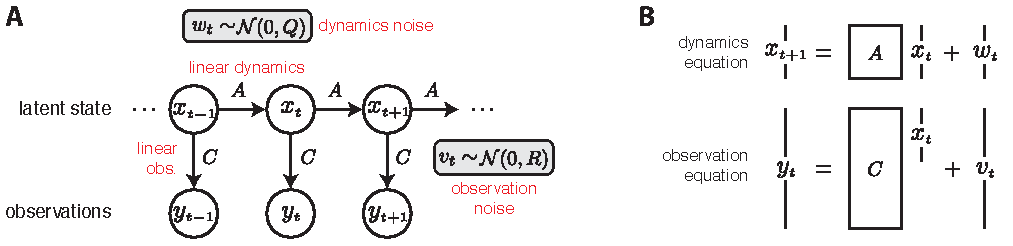
\includegraphics[width=.975\textwidth]{figs/KFgraphicalmodel3}
% \caption{Two regimes of behavior: noisy dynamics and noisy observations}
% \label{fig:graphicalmodel}
% \end{figure}

\section{Notes}

\subsection{Other topics to include}

\begin{itemize}
\item subspace fitting methods 
\item reduced versions: diagonal $R$ or noiseless setting: $R=\epsilon
  I$ (which is DMD).  $C=0 \implies$ no dynamics (Gaussian
  mixture model).
\end{itemize}

\subsection{Things to cite:}
\begin{itemize}
\item Liam's ``new look'' paper \cite{Paninski10}
\item Lars' NIPS paper on spectral methods \cite{Buesing2012neurips}
\item Byron's paper on GPFA \cite{BYu09}.
\item Byron Yu's KF notes \cite{BYutechreport04}.
\item Max Welling's notes \cite{Welling10}. 
\item KF tutorials: \cite{Faragher12,Barker95}.
\item Book on classical non-Bayesian treatment: \cite{Sayed11book}.
\item Book on Bayesian treatment: \cite{SarkkaBook2013}.
\end{itemize}

%========= APPENDIX ======================= 
%\setcounter{section}{0}


\begin{appendices}

\section{Standard Kalman Filtering Equations}
 
Here we provide the ``standard'' Kalman filtering equations, which
differ from those provided in the main text
(eqs.~\ref{eq:KFprior}-\ref{eq:KFcov}) and rely on a quantity known as
the {\it Kalman gain}. These formulas can be derived from the Kalman
filtering equations in the main text using the matrix inversion lemma
(eq.~\ref{eq:mil}), and thus result in identical values for the mean
and covariance of the latent state.

However, it should be noted that these ``standard'' updates require
the inversion of an $n\times n$ matrix on each time step (where $n$ is
the dimensionality of the observations $\vy$), whereas the updates in
the main text require inverting a matrix of size $m \times m$ (where
$m$ is the dimensionality of the latent state $\vx$).  It is thus
unclear to this author why standard texts seem to favor the version of
the Kalman filtering equations provided here.


The ``standard'' Kalman filtering equations are given by:
{\bf Step 1 (Prediction):}
\begin{alignat}{2}
\mu_{t*} &\;=\; A\mu_{t-1}    & &   \textrm{(KF prior mean)}  \label{eq:priormean}\\ 
V_{t*} &\;=\; AV_{t-1}A\trp + Q    & &   \textrm{(KF prior
  covariance)}  \label{eq:priorcov}\\
\intertext{\bf Step 2 (Update):}
K_t &\;=\; V_{t*}C\trp (CV_{t*}C\trp + R)\inv   & &    \textrm{(Kalman gain)}  \label{eq:kfgain}\\
\mu_t &\;=\;  \mu_{t*} + K_t (\vy_t - C\mu_{t*}) \qquad & &
\textrm{(KF posterior mean)} \label{eq:meanupdate}\\
V_t &\;=\; V_{t*} - K_t (CV_{t*}C\trp + R) K_t\trp  \quad & &
\textrm{(KF posterior
  covariance)}. \label{eq:covupdate}
 \end{alignat}


 % The Kalman Filtering equations given in Sec.~\ref{sec:KF} can be
 % manipulated to obtain these ``standard'' formulas for the Kalman filter,
 % which are typically written in terms of the ``Kalman gain'' (for
 % reasons that the author does not fully understand, given that this
 % version is computationally more costly when the number of
 % observations is greater than the number of latent dimensions).

To derive the relationship, we can apply the matrix inversion lemma
 (eq.~\ref{eq:mil}) to the posterior covariance formula from the main text
 (eq.~\ref{eq:KFcov}):
\begin{align}
V_{t} = (V_{t*}\inv +  C\trp R\inv C)\inv 
&= V_{t*} - V_{t*}C\trp (C V_{t*} C\trp + R)\inv C V_{t*} \\
&= V_{t*} - K_{t}   (CV_{t*}C\trp + R) K_t\trp,
\end{align}
where $K_t$ is the Kalman gain defined above (eq.~\ref{eq:kfgain}).

To derive the update formula for the mean
(eq.~\ref{eq:meanupdate}), we start with the original expression for
the mean (eq.~\ref{eq:KFmean}):
\begin{alignat}{2}
  \mu_{t} &= V_{t}(C\trp R\inv \vy_{t} + V_{t*}\inv \mu_{t*}) \\
  &=V_{t}C\trp R\inv \vy_{t} + V_t V_{t*}\inv \mu_{t*}.
\end{alignat}
The first of these terms is equal to:
\begin{align}
  \label{eq:6}
  V_t C\trp R\inv \vy_t &=  (V_{t*} - V_{t*}C\trp (C V_{t*} C\trp +
                          R)\inv C V_{t*}) C\trp R\inv \vy_t \\
                        &=  (V_{t*}C\trp - K_t C V_{t*} C\trp) R\inv \vy_t \\
                        &=  (V_{t*}C\trp (C V_{t*} C\trp + R)\inv (C V_{t*} C\trp + R) - K_t C V_{t*} C\trp) R\inv \vy_t \\
                        &= (K_t (C V_{t*} C\trp + R) - K_t CV_{t*}C\trp) R\inv \vy_t \\
                        &= K_t R R\inv \vy_t \\
                        &= K_t \vy_t.                         \label{eq:kyterm}
\end{align}
The second term is given by:
\begin{alignat}{2}
  V_{t} V_{t*}\inv \mu_{t*}  &= (V_{t*} - K_{t}  C V_{t*}) V_{t*}\inv
  \mu_{t*} \\
  &= \mu_{t*} - K_t C \mu_{t*}. \label{eq:muterm}
\end{alignat}
Summing together the terms in (eq.~\ref{eq:kyterm}) and (eq.~\ref{eq:muterm})
gives the traditional Kalman filtering mean update equation (eq.~\ref{eq:meanupdate}).


 
% \section{Stationary Setting}
% One question we can ask is: if we assume that the parameters $A$, $B$,
% $Q$, $R$, are fixed and therefore not varying in time, what will be the asymptotic value of the
% posterior variance $V_t$ as $t \rightarrow \infty$?  We can address
% this question by noticing that running one full step of the Kalman filter takes us
% from covariance $V_t$ to covariance $V_{t+1}$ at the next time step
% via (combining eqs.~\ref{eq:KFpriorcov} and \ref{eq:KFmean}):
% \begin{equation}
%   \label{eq:1}
% V_{t+1} =   ((AV_{t}A\trp + Q)\inv + C\trp R\inv C)\inv
% \end{equation}
% If we denote by $P$ the covariance of the converged posterior, then we
% can substitue $\Pinf = V_{t+1} = V_t$ into the above equation and
% solve for $P$.  In the restricted case where $A=C=I$
% \begin{align}
%   \label{eq:2}
%   \Pinf\inv &= (\Pinf+Q)\inv + R\inv \\
%   \implies \Pinf +Q &= \Pinf +  \Pinf R\inv (\Pinf+Q) \\
%   \implies \Pinf R\inv \Pinf + \Pinf R\inv Q &= Q
% \end{align}

% {\it: (April 2018): I have no idea where the following came from:}\\
% $\Pinf = (\Pinf+Q)R/(\Pinf+Q+R)$, which yields the solution
% \begin{align}
%   V_\infty &\;=\; \frac{-Q + \sqrt{Q^2 + 4QR}}{2} \\
%            &\;=\;  \frac{Q}{2}
%              (\sqrt{1+4RQ\inv} - 1).
% \end{align}

% Note therefore that if we assume $V_0 = V_\infty$, i.e., that our
% initial variance is equal to the asymptotic posterior variance, then
% prior variance $S$, Kalman gain $K$ and posterior variance $P$ are
% constant. We can therefore simplify the above to simply:
% \begin{equation}
% \mu_t = (1-K) \hat \vx_y{t-1} + K \vy_t, 
% \end{equation}
% where $K$ is the fixed constant:
% \begin{eqnarray} 
% K &=& (Q+P)(Q+P+R)\inv \\
% &=& \frac{1+\sqrt{1+4\frac{R}{Q}}}{1+\sqrt{1+4\frac{R}{Q}} +
%   2\frac{R}{Q}} \\
% %&=& \left(1+2\frac{\frac{R}{Q}}{1+\sqrt{1+4\frac{R}{Q}}}\right)\inv \\
% &=& \left(1+2\left(\tfrac{Q}{R} + \sqrt{\tfrac{Q^2}{R^2} +
%       4\tfrac{Q}{R}}\right)\inv\right)\inv
% \end{eqnarray}
% This makes $\hat
% \vx$ a simple auto-regressively filtered version of $\vy$. We can
% write the matrix version as:
% \begin{equation}
% D\hat \vx = K \vy, 
% \end{equation}
% where $D$ is a bi-diagonal matrix with 1 on the main diagonal and
% $K-1$ on the below-diagonal:
% \begin{equation}
% D = \begin{bmatrix} 1  \\
% K\!-\!1 & 1 \\
%  & \ddots & \ddots \\
% & & K\!-\!1 &  1. 
% \end{bmatrix}
% \end{equation}
% This of course allows us to write
% \begin{equation}
% \hat \vx = D\inv K \vy 
% \end{equation}
% so that we have
% \begin{eqnarray}
% %\hat \vx|\vy &\sim& \Nrm(D\inv K\vy,\; 0) \\
% \hat \vx | \vx &\sim& \Nrm(D\inv K \vx,\; K^2 D\inv R D^{-\top}). \\
% %\hat \vx  &\sim& \Nrm(0,\;  K^2 D\inv(AQA\trp + R)  D^{-\top}).
% \end{eqnarray}


% ===================================    
\section{Incorporating inputs}
\label{asec:inputs}

One common extension to the LLDS model defined in
(eq.~\ref{eq:latent}-\ref{eq:obs}) is to incorporate linear dependence
of both the latents and observations on a set of external inputs
signal $\vu_t\in \RR^d$.  The extended model becomes:
\begin{alignat}{4}
  \vx_{t} &=\; A \vx_{t-1}\; &+& \;B \vu_{t} + \vw_t, \qquad & &\vw_t \sim \Nrm(0,Q)
  \qquad & & \text{\it(latents with inputs)}\\
  \vy_{t} &=\; C \vx_t &+& \; D \vu_t + \vv_t, \qquad & &\vv_t \sim \Nrm(0,R) 
 \qquad & & \text{\it(observations with inputs)}
\end{alignat}
where $B\in \RR^{m \times d}$ and $D\in \RR^{n\times d}$ are matrices
capturing the influence of the inputs on the latents and observations,
respectively.

% ==============================
\subsection{Kalman filter}
% ==============================

The addition of inputs affects the Kalman filter only via its mean.
First, the prior over the latent $\vx_t$ at time step $t$
given previous observations $\vy_{1:t-1}$,  denoted
$\Nrm(\mu_{t*}, V_{t*})$ (eq.~\ref{eq:KFprior}), has an updated mean (eq.~\ref{eq:KFpriormean})
given by:
\begin{alignat}{2}
  \mu_{t*} &= A \mu_{t-1} + B \vu_t, \quad & & \text{\it (prior mean
    w/ inputs)} \label{eq:KFpriormean2},
\end{alignat}
while the prior covariance $V_{t*}$ (eq.~\ref{eq:KFpriorcov}) is
unchanged.  For the first time bin, we now have a non-zero mean: $\mu_{1*} = B\vu_1$.

Second, the inputs affect the posterior mean (the Kalman
filter output) via their influence on observations $\vy_t$.  The
posterior over $\vx_t$ given observations $\vy_{1:t}$, denoted
$\Nrm(\mu_t, V_t)$ (eq.~\ref{eq:KF}), has updated mean given by:
\begin{alignat}{2}
\mu_{t} &= V_{t}(C\trp R\inv (\vy_{t}-D\vu_t) + V_{t*}\inv \mu_{t*}), \qquad
& & \text{\it (Kalman filter mean w/ inputs)}  \label{eq:KFmean2} 
\end{alignat}
where again the covariance $V_t$ (eq.~\ref{eq:KFcov})  remains unchanged.


The marginal likelihood $P(\vy_{1:T})$, which is also computed during
Kalman filtering, is also changed so that the mean of
$\vy_t \mid \vy_{1:t-1}$ incorporates the effect of the inputs.  The
terms in the marginal likelihood (eq.~\ref{eq:margli}) become:
\begin{equation}
  \label{eq:margliterms2}
  P(\vy_t \mid \vy_{1:t-1}) = \Nrm(C\mu_{t*} + D\vu_t, CV_{t*}C\trp + R),
\end{equation}
which is also valid for the first time bin, since $\mu_{1*} =0$ and
$V_{1*} = Q_0$, and thus $P(\vy_1) = \Nrm(D\vu_1, CQ_0C\trp + R)$.

The inclusion of inputs has no affect on the Kalman smoothing
equations.



% =========================================
\subsection{Learning parameters via EM}
% =========================================

The inclusion of inputs enlarges the Gaussian LLDS model parameters to $\theta =
\{A,B,C,D, Q, Q_0, R\}$, and the presence of $B$ and $D$ affect the
EM update equations for all other parameters. 

With inputs, the complete data log-likelihood (eq.~\ref{eq:LCD})
to be computed in the E-step becomes:
\begin{align}
  \label{eq:LCD2}
L_{CD}(\theta) &=  \; \E \left[ \log \Nrm(\vx_1; B\vu_1, Q_0) + \sum_{t=2}^{T} \log \Nrm(\vx_{t};
                  A\vx_{t-1} +B\vu_t,  Q) +  \sum_{t=1}^T \log \Nrm(\vy_t ; C\vx_t+D\vu,R) \right] 
  \\
    % ==================================================
               &=  -\tonehlf \E [(\vx_1-B\vu_1)\trp
                                              Q_0\inv (\vx_1-B\vu_1)]  -
                                              \tonehlf \log |2\pi Q_0|
                                              \nonumber \\
    & \qquad             - \tonehlf \E\left[ \sum_{t=2}^{T} (\vx_{t} - A
      \vx_{t-1}-B\vu_{t})\trp Q\inv (\vx_{t} - A\vx_{t-1}-B\vu_{t}) \right] -\tfrac{T-1}{2} \log |2\pi Q| \nonumber \\
    & \qquad - \tonehlf \E\left[\sum_{t=1}^T (\vy_t - C
    \vx_t-D\vu_{t})\trp R\inv (\vy_t - C\vx_t-D\vu_{t}) \right]
      -\tfrac{T}{2} \log |2\pi R| \\
  % ==================================================
               & =
                 %  - \tonehlf \Tr\left[Q_0\inv M_{(1,1)}  \right]
                 %  - \tonehlf \Tr\left[ Q_0\inv B U_{(1,1)} B\trp \right]
                 % + \Tr\left[Q_0\inv B \tilde U_{(1,1)} \right]
                 %  -\tfrac{1}{2} \log |2\pi Q_0|
                  - \tonehlf \Tr\left[Q_0\inv \left(M_{(1,1)} 
                 -2  B \tilde U_{(1,1)}
                 + B U_{(1,1)} B\trp 
                 \right)\right]
                  -\tfrac{1}{2} \log |2\pi Q_0|
                 -\tfrac{T-1}{2} \log |2\pi Q|
                 -\tfrac{T}{2} \log |2\pi R|
                 \nonumber \\
   & \qquad
     - \tonehlf \Tr\left[Q\inv
     \left( M_{(2,T)} + A M_{(1,T-1)}A\trp  
     +B U_{(2,T)} B\trp
     %\right)
%     \right]
%     \nonumber \\
%
%               & \qquad
%                 + \Tr\left[Q\inv \left(
                 -2 A M_\Delta 
                 -2B \tilde U_{(2,T)}
                 + 2B  \tilde U_{\Delta} A\trp \right)\right]
%
                  \nonumber \\
   & \qquad 
                  - \tonehlf \Tr\left[R\inv  \left( Y  
+C M_{(1,T)} C\trp
     +D U_{(1,T)} D\trp %\right) \right]
     %+ \Tr\left[R\inv \left(
     -2C \tilde Y 
     -2 D U_{\vy} 
     +2 D \tilde U_{(1,T)} C\trp \right)\right]  ,
     \label{eq:cdllwinput}
\end{align}
where the sufficient statistics now correspond to:
\begin{alignat}{4}
  \label{eq:19}
  M_{(t_1,t_2)} &= \sum_{t=t_1}^{t_2} \vm_t \vm_{t}\trp + \Sigma_{t}
  \qquad && 
  U_{(t_1,t_2)} = \sum_{t=t_1}^{t_2} \vu_t \vu_t\trp 
  \qquad &&
\tilde  U_{(t_1,t_2)} = \sum_{t=t_1}^{t_2} \vu_t \vm_{t}\trp 
   \nonumber \\
   M_\Delta  &= \sum_{t=1}^{T-1} \vm_t \vm_{t+1}\trp + \Sigma_{t,t+1}
  \qquad && 
\tilde U_\Delta = \sum_{t=1}^{T-1} \vu_{t+1} \vm_{t}\trp
  \qquad && 
    U_{\vy}  = \sum_{t=1}^{T} \vu_t \vy_{t}\trp
  \nonumber \\
    Y  &= \sum_{t=1}^{T} \vy_t \vy_{t}\trp
  \qquad && 
  \tilde  Y  = \sum_{t=1}^{T} \vm_{t}\vy_t\trp.
\end{alignat}


The M-step updates for the dynamics model weights $A$ and $B$, and for
the observation model weights $C$ and $D$ can now
be computed jointly as:
\begin{align}
  \label{eq:mstepAB} 
  \begin{bmatrix}
    \hat A & \hat B
  \end{bmatrix} &=
                                      \begin{bmatrix}
                                        M_\Delta\trp &
                                        \tilde U_{(2,T)}\trp
                                      \end{bmatrix}
                  \begin{bmatrix}
                    M_{(1,T-1)} & \tilde U_\Delta\trp \\
                    \tilde U_\Delta & U_{(2,T)}
                  \end{bmatrix}\inv
  \\
  \begin{bmatrix}
    \hat C & \hat D
  \end{bmatrix} &=
                  \begin{bmatrix}
                    \tilde Y\trp &
                    U_{\vy}\trp
                  \end{bmatrix}
                  \begin{bmatrix}
                    M_{(1,T)} & \tilde U_\Delta{(1,T)}\trp \\
                    \tilde U_\Delta{(1,T)} & U_{(1,T)}
                  \end{bmatrix}\inv,
\end{align}
where we have ignored the contribution of the very first term to $B$,
since this allows us to eliminate the dependence on $Q$ and $Q_0$ when
computing updates for $A$ and $B$, greatly simplifying the expression
in (eq.~\ref{eq:mstepAB}). This is a small price to pay, however,
since it concerns only the input contribution to the latent vector in
very first time bin.


Finally, the M-step updates for covariances $Q$, $R$, and $Q_0$ are
given by:
\begin{multline}
  \label{eq:QRwinput}
  \hat Q \; =\; \frac{1}{T-1} \Big(  M_{(2,T)} \,+\, \hat A  M_{(1,T-1)}\hat A\trp \,+\,
  \hat B U_{(2,T)}\hat B\trp    \\
\,-\,  \hat A  M_\Delta  \,-\, M_\Delta \trp \hat A\trp
  \,-\, \hat B \tilde U_{(2,T)} \,-\, \tilde U_{(2,T)}\trp \hat B\trp
  \,+\, \hat B  \tilde U_{\Delta} \hat A\trp \,+\, \hat A \tilde U_{\Delta}\trp \hat B\trp
  \Big)
\end{multline}
\begin{multline}
  \hat R \;=\; \frac{1}{T} \Big(  Y \,+\,  \hat C  M_{(1,T)}\hat C\trp \,+\, \hat D
  U_{(1,T)} \hat D\trp
    \\
  \,-\,  \hat C \tilde Y  \,-\, \tilde Y\trp \hat C\trp
  \,-\,  \hat D U_{\vy} \,-\, U_{\vy}\trp \hat D\trp 
 \,+\,  \hat D \tilde U_{(1,T)} \hat C\trp \,+\,  \hat C \tilde U_{(1,T)}\trp \hat D\trp
 \Big)
\end{multline}
\begin{equation}
  \label{eq:mstepq0winput}
  \hat Q_0 = M_{(1,1)} +\hat B U_{(1,1)} \hat B\trp - \hat B \tilde U_{(1,1)} - \tilde
  U_{(1,1)}\trp \hat B\trp. \hspace{3.15in}
\end{equation}

\subsection{Identifiability}

As discussed in Sec.~\ref{subsec:identifiability}, Gaussian LLDS
models are only identifiable up to an (invertible) linear
transformation of the latent space.  When transforming the latent
variables by an arbitary invertible linear transformation $H$,
resulting in new latents $\vx_t' = H \vx_t$, we can obtain an
equivalent model by transforming the input matrix $B$ according to
$B' = H B$.  There is no need to transform $D$.


% ===================================
\section{Combining data from multiple experiments}
% ===================================
\label{asec:multi}

In the main text we have assumed that the data consisted of a single
time series of length $T$.  However, it is common to fit a single LLDS
model to data from multiple experiments, consisting of independent
time series $\{\vy^{(1)}_{1:T_1}, \ldots,
\vy^{(k)}_{1:T_k}\}$ of lengths $T_1, \ldots, T_k$.

As in the original derivation, fitting the model can proceed via EM.
The E-step involves running the Kalman Filter-Smoother on each
independent time series to obtain the posterior mean and covariance of
the latents, which can be performed in parallel across datasets.

For the M-step, we simply sum the complete data log-likelihood
(eq.~\ref{eq:cdllnoinput} or eq.~\ref{eq:cdllwinput}) across datasets
before differentiating and solving for the M-step updates.

For the model without inputs, the M-step updates (originally given in
eq.~\ref{eq:mstepa}-\ref{eq:mstepq0}) become:
\begin{align}
  \label{eq:mstepmulti}
  \hat A &= \left(\sum_{i=1}^kM^{(i)}_\Delta\right)\trp  \left( \sum_{i=1}^kM^{(i)}_{(1,T_i-1)}\right)\inv 
  \\
  \hat C &= \left(\sum_{i=1}^k {\tilde Y}^{(i)}\right)\trp  \left(\sum_{i=1}^k
           M^{(i)}_{(1,T_i)} \right)\inv
  \\
  \hat Q &= \frac{1}{\sum_{i=1}^k (T_i-1)} \left(  \sum_{i=1}^k M^{(i)}_{(2,T_i)}
                                           -  A  M^{(i)}_\Delta
                                           - {M^{(i)}_\Delta}\trp A\trp
                                           + A  M^{(i)}_{(1,T_i-1)}A\trp  \right)  \\
 \hat R &= \frac{1}{\sum_{i=1}^k T_i}  \left(  Y^{(i)}
                                          -  C {\tilde Y}^{(i)}
                                           - ({\tilde Y}^{(i)})\trp  C\trp
                                          + C  M^{(i)}_{(1,T_i)}C\trp
          \right) \\
 \hat Q_0 &= \frac{1}{k} \left( \sum_{i=1}^k M^{(i)}_{(1,1)} \right), 
\end{align}
using sufficient statistics $M^{(i)}$, $M^{(i)}_\Delta$, $Y^{(i)}$,
${\tilde Y}^{(i)}$ computed from each dataset
(eqs.~\ref{eq:suffstats1}-\ref{eq:suffstats2}).

Note that the formulas provided here are the nearly same as using the
original M-step updates (eq.~\ref{eq:mstepa}-\ref{eq:mstepq0}), but
with sufficient statistics replaced by their sums across datasets; the
only exception is the updates for the covariance matrices $Q$, $R$,
and $Q_0$, which must take account of the number of datasets $k$ and
number of time points $T_i$ in each.

Thus, given multiple time series in a model with inputs and parameters
$C$ and $D$, the the M-step updates are identical to those in
Appendix~\ref{asec:inputs} (eqs.~\ref{eq:mstepAB}-\ref{eq:mstepq0winput}),
but with denominators of $\sum_{i=1}^k (T_i-1)$,
$\sum_{i=1}^k T_i$ and $k$ for $Q$, $R$, and $Q_0$, respectively.

% ===================================
\section{Incorporating priors}
% ===================================

The EM algorithm converges to a maximum of the log-likelihood
function.  However, in cases where data is limited relative to the
number of parameters, it may be desirable to regularize our estimates
by incorporating a prior over the model parameters. Mathematically,
this is equivalent to adding a penalty (equal to the log-prior) to the
complete-data log-likelihood.  This penalty will alter the M-step
updates, and the EM algorithm will now converge to a maximum of the
posterior, thereby producing a {\it maximum a posteriori} (MAP)
estimate of the model parameters.

For the dynamics
matrix $A$ and observation matrix $C$, it is straightforward to
incorporate a Gaussian prior, which is equivalent to adding a
quadratic penalty to the complete data log-likelihood.  Suppose we
have zero-mean Gaussian priors:
\begin{align}
  A_{[j,:]} &\sim \Nrm(0, \Lambda_A) \\
  C_{[j,:]} &\sim \Nrm(0, \Lambda_C),  
\end{align}
where $A_{[j,:]}$ is the $j$th row of $A$, $C_{[j,:]}$ is the
$j$th row of $C$, and $\Lambda_A$ and $\Lambda_C$ represent $m\times m$
and $n \times n$ covariance matrices, respectively. 

If we assume we have the same prior over all rows of $A$ and over all
rows of $C$, this is equivalent to adding the terms
$-\tfrac{1}{2} \Tr[A\Lambda_A\inv A\trp]$ and
$-\tfrac{1}{2} \Tr[C\Lambda_C\inv C\trp]$ to the complete data
log-likelihood (eq.~\ref{eq:cdllnoinput}).  The gradients of
the penalized complete-data log-likelihood with respect to $A$ and $C$
are now: 
\begin{align}
  \label{eq:dLdApost}
  % \frac{\partial }{\partial A} L_{CD}&= Q \inv \left(\sum_{i=1}^kM^{(i)}_\Delta\right) \trp - Q\inv A
  %                                      \left(\sum_{i=1}^kM^{(i)}_{(1,T_i-1)}
  %                                      \right) - A \Lambda_A\inv\\
  %   \label{eq:dLdCpost}
  % \frac{\partial }{\partial C} L_{CD}&= R \inv \left(\sum_{i=1}^k {\tilde Y}^{(i)}\right)\trp - R\inv C
  %                                      \left(\sum_{i=1}^k M^{(i)}_{(1,T_i)}\right) - C \Lambda_C\inv,
  \frac{\partial }{\partial A} L_{CD}&= Q \inv M_\Delta\trp - Q\inv A
                                       M_{(1,T-1)}
                                        - A \Lambda_A\inv\\
    \label{eq:dLdCpost}
  \frac{\partial }{\partial C} L_{CD}&= R \inv {\tilde Y}\trp - R\inv C
                                       M_{(1,T)} - C \Lambda_C\inv.
\end{align}
Note that if the dataset consists of $k$
independent time series (as discussed in Appendix~\ref{asec:multi}), then in the above equations we set the sufficient
statistics equal to their sum across datasets, that is:
$M_\Delta = \sum_{i=1}^kM^{(i)}_\Delta$,
$M_{(1:\tau)} = \sum_{i=1}^kM^{(i)}_{(1,\tau)}$, and
$\tilde Y = \sum_{i=1}^k {\tilde Y}^{(i)}$.


If $Q$ or $R$ is diagonal,  then we have the following closed-form
M-step updates for each row of $A$ or $C$:
\begin{align}
  \label{eq:Apostupdate}
\hat A_{[j,:]} &= \left(M_\Delta\trp\right) _{[j,:]} \left(
                 M_{(1,T-1)}+ {Q_{jj}} \Lambda_A\inv\right)\inv 
  \\
  \label{eq:Cpostupdate}
  \hat C_{[j,:]} &= {\left(\tilde Y\trp\right)_{[j,:]}}  \left(
           M_{(1,T)} + {R_{jj}} \Lambda_C\inv\right)\inv,  
\end{align}
where $Q_{ii}$ and $R_{ii}$ indicate the diagonal elements of the
(diagonal) covariances $Q$ and $R$, respectively, and $X_{[j,:]}$
indicates the $j$'th row of a matrix $X$.

Note that if either prior covariance is proportional to the identity,
$\Lambda_A = \sigma_A^2 I$ or $\Lambda_C = \sigma_C^2 I$, then the
penalty temrs above are equal to $\frac{Q_{jj}}{\sigma_A^2} I $ or
$\frac{R_{jj}}{\sigma_C^2} I $, respectively.  This is equivalent to
ridge regression with ridge parameter
$\lambda = \frac{Q_{jj}}{\sigma_A^2}$ or
$\lambda = \frac{R_{jj}}{\sigma_C^2}$, so the updates for each row
are given by:
\begin{align}
  \label{eq:Aridgeupdate}
\hat A_{[j,:]} &= \left(M_\Delta\trp\right) _{[j,:]} \left(
                 M_{(1,T-1)}+ \left(\tfrac{Q_{jj}}{\sigma_A^2}\right)  I\right)\inv 
  \\
  \label{eq:Cridgeupdate}
  \hat C_{[j,:]} &= {\left(\tilde Y\trp\right)_{[j,:]}}  \left(
           M_{(1,T)} + \left(\tfrac{R_{jj}}{\sigma_C^2}\right) I\right)\inv,
\end{align}
although note that the ridge
parameter for each row of $A$ or $C$ differs depending on the noise
variance $Q_{jj}$ or $R_{jj}$ for that latent or observed dimension,
respectively.

In the case that we do not wish to restrict $Q$ or $R$ to diagonal, we
can use Kronecker identities to derive the vectorized M-step update
for $A$ and $C$.  Specifically, we use the identity
$\mvec(ABC) = (C\trp \otimes A) \mvec(B)$, where $\mvec(\cdot)$ is the
``vectorize'' operator that transforms a matrix into a vector by
stacking its columns. With this identity, we can set the partial
derivatives (eqs.~\ref{eq:dLdApost}-\ref{eq:dLdCpost}) to zero and
obtain the following solutions:
\begin{align}
  \label{eq:Avecpostupdate}
  \mvec(\hat A) &=
                           \left(   M_{(1,T-1)} \trp \otimes
                  I + \Lambda_A\inv \otimes  Q
                  \right)\inv 
%
                  \mvec \left(M_\Delta\trp
                \right)
  \\
  \label{eq:Cvecpostupdate}
  \mvec(  \hat C) &=   \left( M_{(1,T)}\trp \otimes I + \Lambda_C\inv
                    \otimes R \right)\inv
                %
                  \mvec\left(\tilde
                  Y \trp
                  \right).
\end{align}
Note that these solutions require inverting an $m^2 \times m^2$ matrix
for $\hat A$ and and an $mn \times mn$ matrix for $\hat C$, which have
computational costs of $O(m^6)$ and $(Om^3n^3)$, respectively. This
may be prohibitive when the latent dimensionality $m$ or observation
dimensionality $n$ is large.  In such cases, it may be more efficient
to use conjugate gradient methods to numerically minimize (or
approximately minimize) the complete-data log-likelihood for $A$ and
$C$ using the gradients in (eqs.~\ref{eq:dLdApost}-\ref{eq:dLdCpost}).

\subsection{Priors for the LLDS model with inputs}
{\it To add:  priors on $A$, $B$, $C$, $D$}


% ===================================
\section{Speeding up inference}
% ====================p===============

Describe how to speed up inference for long time series, namely by avoiding matrix inversions once the covariance has stabilized; this dramatically speeds up the Kalman Filter-Smoother.

Also mention Martens paper on ASOS \citep{Martens2010LDS}.


% ===================================
\section{Structured assumptions}
% ===================================
{\it to add}

\subsection{Diagonal covariances}
{\it to add}

\subsection{Diagonal input weights}

{\it to add}

\subsection{Block structure in $A$}
{\it to add}
%===================================
\section{Missing data}
% ===================================

{\it to add}    
% ===================================
\section{Implementation using block-sparse matrices}
% ===================================

Here we describe the LLDS model using block-sparse matrices and
vectors of concatenated observations and latents, which facilitates
efficient computations of marginal likelihood and posterior
distribution.

\subsection{Expressing the model with block-sparse matrices}

Let us begin by stacking the latents $\{\vx_t\}$, observations
$\{\vy_t\}$, latent noise $\{\vw_t\}$, and observed noise $\{v_t\}$
for all time steps $t \in \{1, \ldots, T\}$ into four gigantic column
vectors $\vx$, $\vy$, $\vw$, $\vx$, respectively.  Thus, for example,
we have
\begin{equation}
  \label{eq:18}
  \vx = \begin{bmatrix}
    \vx_1 \\ \vdots \\ \vx_T 
  \end{bmatrix}.
\end{equation}
Then we can rewrite the LLDS model in matrix form:
\begin{align}
  \label{eq:Dx}
  \mH \vx &=  \vw  \\
  \label{eq:y}
\vy &= \mC \vx + \vv, 
\end{align}
where $\mH$ is a block bi-diagonal matrix given by
\begin{equation}
\mH = \begin{bmatrix}
  I \\
-A & I \\
  & -A  & I \\
 & & \ddots & \ddots \\ 
 & &  & -A  & I
\end{bmatrix},
\end{equation}
constructed so that the $t$'th row-block expresses the condition that
$\vx_t - A\vx_{t-1} = \vw_t$, and $\mC$ is a block diagonal matrix
with copies of the observation matrix $C$ along the main diagonal:
\begin{equation}
\mC =   I_{T} \otimes C   \triangleq \begin{bmatrix}
C \\
& \ddots \\
& & C 
\end{bmatrix},
\end{equation}
where $ I_T \otimes C$ denotes Kronecker
product between the $T \times T$ identity matrix and $C$.

We can also compactly write the distributions over the noise vectors:
\begin{alignat}{2}
  \label{eq:w}
  \vw &\sim \Nrm(0,\mQ),  \quad  & \mQ &=
%   \begin{bmatrix}
%     Q_0 & 0 \\ 
% 0 &   I_{T-1} \otimes Q 
%   \end{bmatrix}\\
  \begin{bmatrix}
    Q_0 & \\ 
    &  Q & \\
    & & \ddots \\
    & & & Q
  \end{bmatrix}\\
\vv &\sim \Nrm(0,\mR), \quad  & \mR &= I_T \otimes R, 
\end{alignat}
where the block structure of $mQ$ accounts for the fact that $Q_0$ is
the prior over the initial latent.

\subsection{Prior, Conditional, Posterior, \& Marginal}

Now, we can derive a simple expressions for the prior, conditional, marginal
and posterior distributions.

First, the dynamics equation (eq.~\ref{eq:Dx}) and the distribution for
latent noise $\vw$ (eq.~\ref{eq:w}) implies that
$\mH\vx \sim \Nrm(0,\mQ)$.  This implies that we can write the prior
over the latent as a linear transformation of the latent noise:
\begin{align}
  \label{eq:xprior}
  \vx  &\sim \Nrm(0, \tilde \mQ),  \qquad \text{\it (prior)} \\
  \tmQ &=
  \mH\inv \mQ \mH\trpinv =  (\mH\trp {\mQ}\inv \mH)\inv.
\end{align}
While the prior covariance $\tmQ$ is a full $mT \times mT$ matrix, the
right-most expression on the second line shows that its inverse
$\tmQ\inv$ is the block-tridiagonal matrix $\mH\trp \mQ \inv \mH$, which
is requires only linear memory in $T$.

Second, the observation equation (eq.~\ref{eq:y}) implies that the conditional distribution of $\vy$ given $\vx$ can be written
\begin{align}
  \label{eq:ycondx}
  \vy\mid \vx &\sim \Nrm(\mC\vx,\mR).  \qquad \text{\it (conditional)}
\end{align}
This allows us to apply the generic formula for linear-Gaussian
systems (Gaussian Fun Fact \#4, eq.~\ref{eq:gfflingauss}), which
implies that the posterior distribution (which is also the output of
the Kalman smoother) is:
\begin{equation}
  \label{eq:post}
  \vx \mid \vy = \Nrm \Big( (\mC\trp \mR\inv \mC + \tmQ\inv)\inv
  \mC\trp \mR\inv \vy  , (\mC\trp \mR\inv \mC +
  \tmQ\inv)\inv\Big). \qquad \text{\it (posterior)}
\end{equation}
Note that the posterior covariance is a full matrix, but its inverse
is once-again tri-diagonal.

Finally, the marginal likelihood can be derived by observing that
$\vy$ is a linear transformation of $\vx$ plus Gaussian noise
(Gaussian fun fact \#1, eq.~\ref{eq:gfflin}):
\begin{equation}
  \label{eq:margliMatrix}
\vy \sim \Nrm(0,\mC \tmQ  \mC\trp + \mR). \qquad \text{\it (marginal)}
\end{equation}

\subsection{Efficient evaluation}
\label{sec:blocksparseeval}
\textbf{Log marginal likelihood}
%\label{sec:logmargli}

The log of the marginal-likelihood (eq.~\ref{eq:post}), which is used for
fitting $\theta$ or evaluating test performance, can be written
explicitly as:
\begin{equation}
  \label{eq:logmargliMatrix}
  \log P(\vy) = -\tonehlf \log | \mLam| - \tonehlf  \vy\trp \mLam\inv
  \vy  - \tfrac{T}{2}\log (2\pi),  \qquad \text{\it (log marginal likelihood)}
\end{equation}
where $\mLam = \mC \tmQ \mC\trp + \mR$ is the marginal covariance of
$\vy$ given $\theta$.  However, $\mLam$ is a $mT \times mT$ matrix,
which requires $O(m^2T^2)$ storage and $O(m^3T^3)$ computational cost
to invert, which is infeasible for even medium-length datasets.

We can achieve dramatically higher efficiency by exploiting the
special block-diagonal structure of the matrices $\mC$, $\mR$, and
$\tmQ\inv$. First, we can use the matrix inversion lemma
(eq.~\ref{eq:mil}) to write the inverse covariance:
\begin{equation}
  \label{eq:3}
  \mLam\inv = (\mC \tmQ \mC\trp + \mR)\inv = \mR\inv - \mR\inv \mC (
  \tmQ\inv + \mC\trp \mR\inv \mC)\inv \mC\trp \mR\inv.
\end{equation}
This allows us to evaluate the quadratic term in (eq.~\ref{eq:logmargliMatrix}) as:
 \begin{equation}
 \vy\trp \mLam\inv \vy =  \vy\trp \mR\inv \vy  -  \vy\trp \mR\inv  \mC (
 \tmQ\inv + \mC\trp \mR\inv \mC)\,  \backslash\,  (\mC\trp \mR\inv \vy),
 \qquad \text{\it (quadratic term)}
 \label{eq:4}
\end{equation}
where `$B \backslash A$' denotes ``matrix left divide'' of $A$ by $B$,
which can be implemented via \texttt{ B $\backslash$ A} in Matlab, and
by \texttt{numpy.linalg.solve(A,B)} in python.  This operation is
equivalent to $B\inv A$, but far more efficient as it does not require
explicitly forming the inverse of $B$, and is only $O(T)$ complexity
for the block-tridiagonal matrix $(\tmQ\inv + \mC\trp \mR\inv \mC)$.

Secondly, we can use the matrix-determinant lemma (eq.~\ref{eq:mdl})
to efficiently evaluate the log-determinant term in
(eq.~\ref{eq:logmargliMatrix}):
\begin{align}
  \label{eq:5}
  \log |\Lambda| &= \log |\mC \tmQ \mC\trp + \mR| = \log \left(|\tmQ| |\mR| | 
                   \tmQ\inv + \mC\trp \mR\inv   \mC
                   | \right) \nonumber \\
  &= - \log |\tmQ\inv | - \log |\mR| + \log |
    \tmQ\inv + \mC\trp \mR\inv \mC|,
     \qquad \text{\it (log-determinant term)}
\end{align}
where $\mR$ is block-diagonal and $\tmQ\inv$ and $(\tmQ\inv  +
\mC\trp\mR\inv \mC)$ are both block-tridiagonal matrices whose determinants can
be obtained in $O(T)$ time.

\textbf{Posterior mean and covariance}
%\asubsubsection{Posterior mean and covariance}
%\label{sec:postcov}

We can efficiently compute the posterior mean over the latents given
the data (eq.~\ref{eq:post} by once again using the `backslash'
operator to avoid explicitly inverting an $mT \times mT$ matrix:
\begin{equation}
  \label{eq:postmean}
  \E[\vx \mid \vy] = (\mC\trp \mR\inv \mC + \tmQ\inv)\, \backslash\,
  \mC\trp \mR\inv \vy. \qquad \text{\it (posterior mean)}
\end{equation}


As noted above, the posterior covariance over the latents given the
data, $(\mC\trp \mR\inv \mC + \tmQ\inv)\inv$, is a full $mT \times mT$
matrix, but its inverse, $\mC\trp \mR\inv \mC + \tmQ\inv$, is
symmetric and block-tridiagonal.  We can exploit this structure to
efficiently compute the main and above-diagonal blocks of the
posterior covariance, which are useful for quantifying uncertainty in
the latents or for the EM algorithm discussed below.

Specifically, the diagonal blocks $\Sigma_t$ and immediate above-diagonal
blocks $\Sigma_{t,t+1}$ of the posterior covariance %$(\mC\trp \mR\inv
% \mC + \tmQ\inv)\inv$
can be computed in linear time via an efficient recursion
\cite{Rybicki91}.  A Matlab implementation of this algorithm is
available at \url{https://github.com/pillowlab/invBlockTriDiag}.


% =========================================
\subsection{Incorporating inputs}
% =========================================

Let $\vu_x$ denote the vector
obtained by vectorizing and stacking the linearly projected inputs $B\vu_t$ from all
time bins, and $\vu_y$ denote the vector obtained by vectorizing and
stacking the linearly projected inputs $D\vu_t$ from all time bins.

With inputs, the prior on the vectorized latents (eq.~\ref{eq:xprior}) becomes
\begin{equation}
  \label{eq:22}
  \vx \sim \Nrm(\mH\inv\vu_x,  \tmQ),
\end{equation}
the conditional distribution of the observations (eq.~\ref{eq:ycondx})
becomes
\begin{align} 
  \label{eq:}
  \vy\mid \vx &\sim \Nrm(\mC\mH\inv\vx+\vu_y,\mR),
\end{align}
and the posterior over the latents (eq.~\ref{eq:post}) becomes
\begin{equation}
  \label{eq:postInput}
  \vx \mid \vy = \Nrm \Big( \, \mSig \big(
  \mC\trp \mR\inv (\vy-\vu_y) +  \tmQ\inv \vu_x \big) \, , \,  \mSig \, \Big),
\end{equation}
where the posterior covariance $\mSig =  (\mC\trp \mR\inv \mC +
  \tmQ\inv)\inv$ is unchanged from the version of the model without inputs.


Finally, the marginal likelihood (eq.~\ref{eq:margliMatrix}) becomes:
\begin{equation}
  \label{eq:margliMatrixInput}
\vy \sim \Nrm(\mC \mH\inv \vu_x + \vu_y,\mC \tmQ  \mC\trp + \mR).
\end{equation}

    

% ====================================================%
\section{ Useful Identities}
% ====================================================%

\subsection{Gaussian Fun Facts}
Here we provide a list of Gaussian identities or ``fun facts'', which
are useful for the derivations in the paper. 
\label{sec:gff}

% ===========================%
{\bf  Fact 1: Sums.}
\begin{alignat}{2}
&\qquad&  x &\sim \Nrm(a,A),  \quad y \sim  \Nrm(b,B) \nonumber \\
\implies & \qquad& x+y & \sim \Nrm(a+b,A+B).
\label{eq:gffsum}
\end{alignat}

% ===========================%
{\bf  Fact 2: Linear Transformations.}
\begin{alignat}{2}
&\qquad&  x &\sim \Nrm(a,A),\quad 
y =Cx \nonumber \nonumber \\
\implies & \qquad& y & \sim \Nrm(Ca, CAC\trp ).
\label{eq:gfflin}
\end{alignat}

% % ===========================%
% {\bf  Fact 3: Linear Measurements}

% \it{(Note to self: do we need this one?)}

% \begin{alignat}{2}
% \text{If}&\; &  Cx &\sim \Nrm(a,A), \nonumber \\
% %\intertext{then if $(C\trp A\inv C)$ is invertible,}
% \text{then if $(C\trp A\inv C)$ is invertible:}& &
% x & \sim \Nrm\Big((C\trp A\inv C)\inv C\trp A\inv a,\;
%  (C\trp A\inv C)\inv \Big),  \\
% %\intertext{or if $C$ itself is invertible},
% \text{or if $C$ is invertible:}
%  & & x & \sim \Nrm\Big( C\inv a,\;  C\inv\! A\, C^{-\!\top} \Big).
% \end{alignat}

% ===========================%
{\bf  Fact 3: Products of Gaussian densities.}
\label{eq:gffprod}
\begin{gather}
\Nrm(a,A) \cdot \Nrm(b,B) \propto \Nrm(c,C)  \\
\text{ where } \quad C = (A\inv+B\inv)\inv, \quad c = C(A\inv a +
B\inv b). \nonumber 
\end{gather}

% ===========================%
{\bf  Fact 4: Conditionals.}

\begin{align}
\textrm{If} \quad 
  \begin{bmatrix} 
x \\ y
  \end{bmatrix} &\sim \Nrm \left( 
    \begin{bmatrix}
      a \\ b
    \end{bmatrix}, 
    \begin{bmatrix}
      A & C \\ C^T & B
    \end{bmatrix}
\right) \nonumber \\ 
\text{ then }
\quad 
x\mid y &\sim \Nrm\left(a+CB\inv(y-b), A-CB\inv C\trp\right) \nonumber  \\
  y \mid x &\sim \Nrm \left(b+C\trp A\inv(x-a), B-C\trp A\inv C \right).
             \label{eq:gffcond}
\end{align}

% ===========================%
{\bf  Fact 5: Expectations of quadratic forms}
\begin{alignat}{2}
  &\qquad&  x &\sim \Nrm(a,A)  \nonumber \\[.5em]
 \text{then}& \qquad&
 \E[ (x-b)\trp B (x - b)] &= (a-b)\trp B (a-b) + \Tr[BA]  \nonumber \\
& & & = \Tr[B (a-b)(a-b)\trp + BA].
   \label{eq:gffqexp} 
\end{alignat}



% ===========================%
{\bf Fact 6: The Linear-Gaussian model.}

Here we consider a linear-Gaussian system defined by a Gaussian prior
over a latent variable $x$, which is transformed linearly and
corrupted by additive Gaussian noise to obtain an observation $y$:
\begin{align}
 x &\sim \Nrm(a,A) \\
  y &=Cx + n , \quad   n  \sim \Nrm(0,R),
\end{align}
where the second equation is equivalent to writing
$ y \mid x \sim \Nrm(Cx,R)$.
First, we can use the Gaussian fun facts above
(eq.~\ref{eq:gffsum}-\ref{eq:gfflin}) to obtain the marginal
distribution over $y$:
\begin{equation}
  \label{eq:13}
  y \sim \Nrm(Ca, CAC\trp + R)
\end{equation}
We can also use ``completing the square'' to derive the posterior
distribution over $x$ given $y$:
% \intertext{and by Bayes' rule, the posterior distritbution is:}
\begin{align}
  x \mid y & \sim \Nrm(d,D), \label{eq:gfflingauss}
\end{align}
% \intertext{where covariance and mean are given by}
where covariance and mean are given by
\begin{equation}
 D = (C\trp R\inv C + A\inv)\inv, \quad 
   d = D  (C\trp R\inv y +A\inv a).
\end{equation}

Lastly, the joint distribution over $x$ and $y$ is given by:
\begin{equation}
  \label{eq:14}
  \begin{bmatrix}
    x \\ y
  \end{bmatrix} = \Nrm \left(
    \begin{bmatrix}
      a \\ Ca 
    \end{bmatrix},
    \begin{bmatrix}
      A & AC\trp  \\
      CA & C A C\trp + R
    \end{bmatrix}
    \right).
\end{equation}

%  These expressions can be derived by a standard approach known as
% ``completing the square'', which involves taking quadratic terms from
% the two exponentials and re-writing their sum as a single quadratic
% expression of the form $(x-d)\trp D\inv (x-d) + const$.


\subsection{Matrix Identities}

% ===========================%
{\bf   Matrix Inversion Lemma}

If $A$ and $B$ are invertible matrices, then:
\begin{equation}
      \label{eq:mil}
(A\inv + X B\inv X\trp)\inv  = A - A X(B+X\trp A X)\inv X\trp A  
\end{equation}

% ===========================%
{\bf   Matrix Determinant Lemma}

If $A$ and $B$ are invertible matrices, then:
\begin{equation}
    \label{eq:mdl}
  \det |A + X B X\trp|  = \det|A| \det|B| \det |X \trp A\inv X + B\inv|
\end{equation}

% ========================= %
{\bf ``Inverse-Flip'' identity}
\begin{equation}
   \left(A^{\top} A+B\inv\right)\inv A^{\top} = BA\trp (ABA^{\top} + I)\inv
\end{equation}
    Proof: Factor $(A\trp A B A\trp + A\trp)$ two different ways to obtain: $A\trp (ABA\trp + I) = (A\trp
    A + B\inv) B A\trp$.  Now, on both sides, multiply on the left by $(A^T A + B\inv)\inv$ and on the right by $(ABA\trp + I)\inv$, and we have the identity.

\end{appendices}
 
\bibliographystyle{unsrt} 
\bibliography{latexstuff/jpbib.bib}
%\bibliography{/Users/pillow/Dropbox/Docs/text/jpbib.bib}

%%%%%%%%%%%%%%%%%%%%%%%%%%%%%% 
\end{document}

